\chapter[Computer-based Mechanisms and Procedures to Gamify CL Sessions]{Computer-based Mechanisms and Procedures to Gamify Collaborative Learning Sessions}
\label{chapter:computer-based-mechanisms-procedures} 

The purpose of this chapter is to show how the ontology OntoGaCLeS, and the GIMF model, presented in previous chapters, can be used in intelligent theory-aware systems to gamify CL sessions, and thus, to deal with the motivation problem caused by the scripted collaboration. 
The \autoref{sec:conceptual-flow-gamify-cl-sessions} presents a conceptual flow to gamify CL sessions proposed as a computer-based procedure that should be used by intelligent theory-aware systems to extract knowledge encoded in the ontology OntoGaCLeS, and then to provide suggestions based on theoretical justification. 
In \autoref{sec:reference-architecture}, a reference architecture based on the conceptual flow to gamify CL sessions is presented. This architecture has been proposed to support the building of computer-based mechanisms that provide support in intelligent-theory aware systems for dealing with the motivation problem caused by the scripted collaboration.

Part of the work described in this chapter was published by the author of this PhD thesis dissertation in the scientific articles:

\begin{itemize}
\item
\aspas{\emph{An Ontology Engineering Approach to Gamify Collaborative Learning Scenarios}} published in the 20\textsuperscript{th} International Conference on Collaboration and Technology, CRIWG 2014, held in Santiago, Chile \cite{ChallcoMoreiraMizoguchiIsotani2014}.

\item
\aspas{\emph{Gamification of Collaborative Learning Scenarios: Structuring Persuasive Strategies Using Game Elements and Ontologies}} published in the 1\textsuperscript{st} International Workshop on Social Computing in Digital Education, SocialEdu 2015, held in Stanford, CA, USA \cite{ChallcoMizoguchiBittencourtIsotani2015}.
\end{itemize}

%%%%%%%%%%%%%%%%%%%%%%%%%%%%%%%%%%
\section[Conceptual Flow to Gamify CL Sessions Using the Ontology OntoGaCLeS]{Conceptual Flow to Gamify Collaborative Learning Sessions Using the Ontology OntoGaCLeS}
\label{sec:conceptual-flow-gamify-cl-sessions}


To avoid the motivation problem caused by the scripted collaboration by means of the gamification, as was mentioned before (in \autoref{chapter:general-background}), it is necessary to solve the context-dependency related to the participants' individual characteristics and traits, and the context-dependency related to the non-game context and target behaviors being gamified. Thus, the gamification should be applied in CL sessions that are the most concrete level of CL scenarios in which the content-domain and participants are well defined, with clear and well-establish group members, CL roles and sequencing of actions to be performed by the group members. 

\autoref{fig:conceptual-flow-gamify-cl-sessions} shows the conceptual flow proposed to gamify CL sessions using the ontology OntoGaCLeS. This flow has been developed from the viewpoint of an instructional designer who employs suggestions given by intelligent-theory aware systems, which in turn use the knowledge encoded in the ontology OntoGaCLeS as a source of information to provide these suggestions.

\begin{figure}[htb]
 \caption{Conceptual flow to gamify collaborative learning sessions using the ontology OntoGaCLeS}
 \label{fig:conceptual-flow-gamify-cl-sessions}
 \centering
 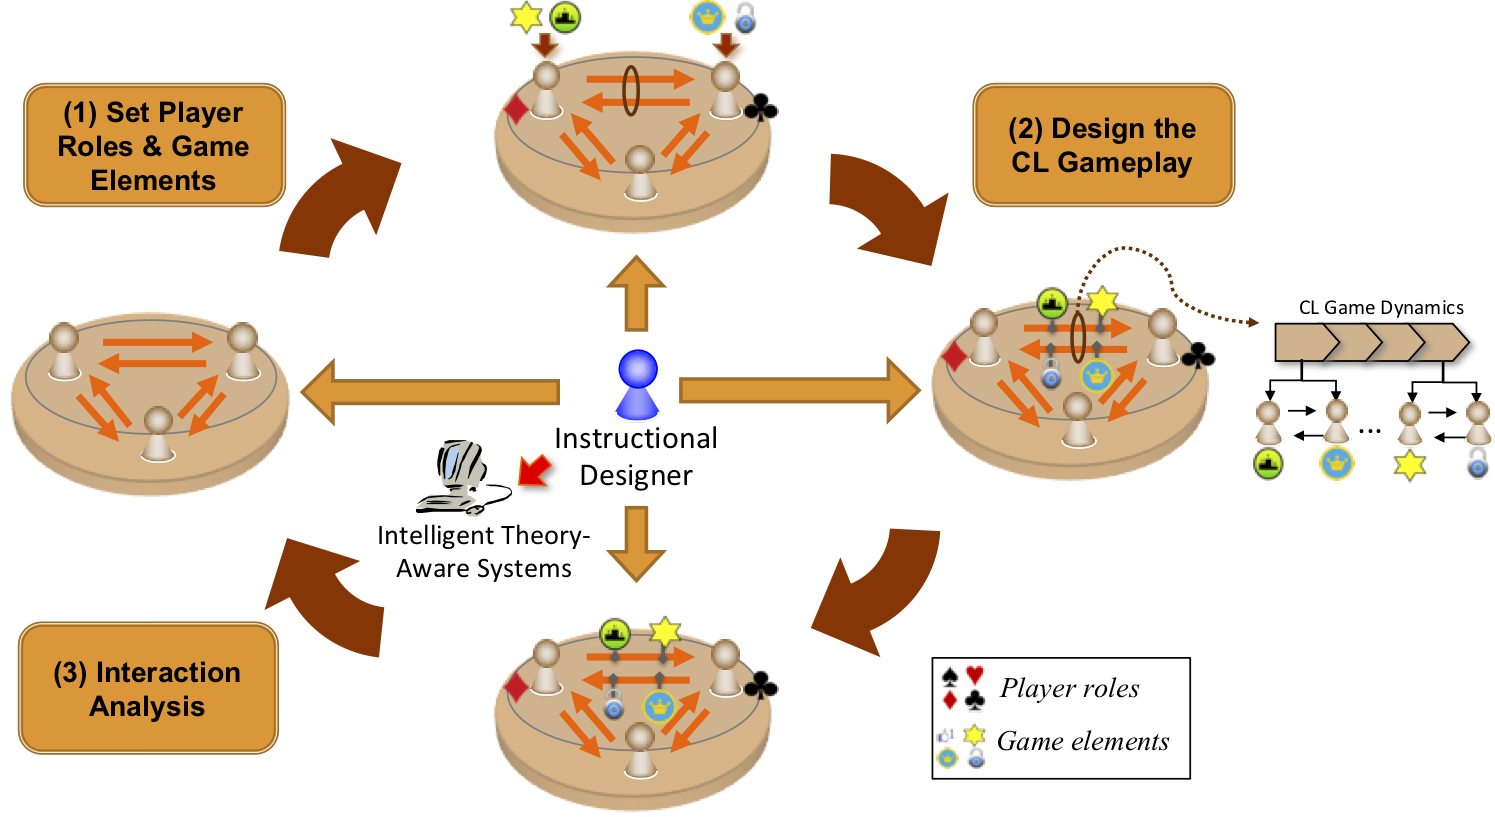
\includegraphics[width=1\textwidth]{images/chap-mechanisms-procedures/conceptual-flow-gamify-cl-sessions.png}
 \fautor
\end{figure}

The basic steps that should be accomplished in the conceptual flow to gamify CL sessions by intelligent-theory aware systems are:

\begin{description}
\item[Step (1):] to set \emph{player roles} and \emph{game elements} for each participant in the CL session,
\item[Step (2):] to design the \emph{CL gameplay} for the CL session, and
\item[Step (3):] to perform an \emph{interaction analysis} over the obtained gamified CL sessions.
\end{description}

\subsection*{Step (1): Set Player Roles \& Game Elements}

For each participant in the CL session, an intelligent theory-aware system that uses the ontology OntoGaCLeS to gamify CL sessions should set the player roles and game elements to solve the context-dependency of gamification related to the participants' individual characteristics and traits. The information of player roles and game elements is extracted from ontology-based models to personalize gamification in CL scenarios based on player types models, so that ontological structures to represent gamified CL scenarios (\autoref{subsec:gamified-cl-scenario}) are used to give suggestions in the identification of player roles and game elements that can be assigned for the participants of a CL session.

\autoref{algorithm:set-player-roles-game-elements} is described in a narrative form as follows:

\begin{itemize}
\item
From \aspas{\emph{an ontology-based model to personalize gamification in CL scenarios based on player types models}} ($ontModel$), the algorithm selects a set of gamified CL scenarios ($setGamifiedCLscenarios$) that would lead the CL role holders of a CL session to internalize the motivation and satisfy their current motivational needs. This step is accomplished by looking the individual motivational goal (\emph{I-mot goal (I)}) in the individual motivational strategies of (\emph{Y<=I-mot goal}) from ontological structures to represent gamified CL scenarios defined as part of the ontology-based model ($ontModel$).

\item
In the set of gamified CL scenarios ($setGamifiedCLscenarios$), the algorithm checks the necessary conditions to assign the player roles \aspas{\emph{I-player role}, and \emph{You-player role}} for the CL role holders who have the potential to become player role holders in each gamified CL scenario ($g$), and the algorithm establishes a priority queue of gamified CL scenarios ($q$) based on the number of desired conditions that are satisfied by the CL role holders who have the potential to become player role holders. If any CL role holder cannot be assigned to any player role, the gamified CL scenario ($g$) is not added to the priority queue ($q$).

\item 
The algorithm sets the player roles for the CL role holders of CL session if no one restriction is violated in the motivational strategy (\emph{Y<=I-mot goal}) of gamified CL scenario ($g$) with highest priority in the queue ($q$).

\item
The algorithm sets the proper game elements for the CL role holders using the structure \aspas{\emph{Gameplay strategy}} (\emph{I-gameplay})
\end{itemize}

\newpage
\begin{algoritmo}
\caption{Algorithm to set player roles and game elements in a CL session}
\label{algorithm:set-player-roles-game-elements}
\begin{algorithmic}[1]\tiny
\Procedure{Setup\_Player\_Roles\_and\_Game\_Elements}{$session$, $ontModel$}
  \begin{tiny}
  \LeftComment{Selecting the scenarios that would lead the CL role holders to achieve their ind. mot. goals}
  \end{tiny}
  \State $setGamifiedCLscenarios \gets$ \{ \}
  \ForAll{$g$ in $ontModel$}
    \State $setIndMotGoals \gets$ getPotentialPlayer($g$, \aspas{Motivational strategy}, \aspas{I-mot goal (I)})
    \ForAll{$p$ in getRoleHolders($session$, \aspas{CL Role Holder})}
      \If{getIndMotGoal($p$) in $setIndMotGoals$} add($setGamifiedCLscenarios$, $g$)
      \EndIf
    \EndFor
  \EndFor
  \begin{tiny}
  \LeftComment{Checking the necessary conditions to assign player roles, and setting the priority using the desired conditions}
  \end{tiny}
  \State $q \gets [ ]$
  \ForAll{$g$ in $setGamifiedCLscenarios$}
    \State $n, c \gets 0$
    \ForAll{$r$ in getRoles($g$, \aspas{Motivational strategy}, sub = \aspas{I-player role})}
      \State $nconds \gets$ getPotentialPlayer($r$, \aspas{Necessary conditions})
      \State $dconds \gets$ getPotentialPlayer($r$, \aspas{Desired conditions})
      \ForAll{$p$ in getRoleHolders($session$, $r$.PotentialPlayer)}
        \If{satisfyAllConditions($p$, $nconds$)}
          \State $n \gets n+1$
          \State $c \gets c+$nroSatisfiedConditions($p$, $dconds$)
        \EndIf
      \EndFor
    \EndFor
    \ForAll{$r$ in getRoles($g$, \aspas{Motivational strategy}, sub = \aspas{You-player role})}
      \State $nconds \gets$ getPotentialPlayer($r$, \aspas{Necessary conditions})
      \State $dconds \gets$ getPotentialPlayer($r$, \aspas{Desired conditions})
      \ForAll{$p$ in getRoleHolders($session$, $r$.PotentialPlayer)}
        \If{satisfyAllConditions($p$, $nconds$)}
          \State $n \gets n+1$
          \State $c \gets c+$nroSatisfiedConditions($p$, $dconds$)
        \EndIf
      \EndFor
    \EndFor
    \If{$n > 0$} insert\_with\_priority($q$, $g$, $<n,c>$)
    \EndIf
  \EndFor
  \begin{tiny}
  \LeftComment{Setting player roles if no one restriction is violated in the ind. mot. strategy}
  \end{tiny}
  \State $g \gets $null; $player\_roles \gets [$ $][$ $]$
  \While{not is\_empty($q$) and is.null($g$)}
    \State $g \gets$ pull\_highest\_priority\_element($q$)
    \ForAll{$p$ in getRoleHolders($session$, \aspas{CL Role Holder})}
      \ForAll{$ms$ in get($g$, \aspas{Motivational strategy})}
%        \State $irole \gets$ 
%        \State $yrole \gets$ 
        \State $prole \gets$ getBestPlayerRole($p$, getRole($ms$, sub = \aspas{I-player role}), getRole($ms$, sub = \aspas{You-player role}))
        \State add($player\_roles \gets [p]$, $prole$)
%        Function getPlayerRole
%        \State $irole \gets$ getRole($ms$, sub = \aspas{I-player role})
%        \State $inconds \gets$ getPotentialPlayer($irole$, \aspas{Necessary conditions})
%        \State $idconds \gets$ getPotentialPlayer($irole$, \aspas{Desired conditions})
%        \State $yrole \gets$ getRole($ms$, sub = \aspas{You-player role})
%        \State $ynconds \gets$ getPotentialPlayer($yrole$, \aspas{Necessary conditions})
%        \State $ydconds \gets$ getPotentialPlayer($yrole$, \aspas{Desired conditions})     
%        \If{satisfyAllConditions($p$, $inconds$) and satisfyAllConditions($p$, $ynconds$)}
%          \If{nroSatisfiedConditions($p$, $idconds$) > nroSatisfiedConditions($p$, $ydconds$)}
%	   \State setRoleHolder($p$, $g$, $ms$, $irole$)
%	 \Else
%  	   \State setRoleHolder($p$, $g$, $ms$, $yrole$)
%          \EndIf
%          \State continue next;
%       \EndIf
%       
%       \If{satisfyAllConditions($p$, $inconds$)}
%	setRoleHolder($p$, $g$, $ms$, $irole$)
%       \EndIf
%       \If{satisfyAllConditions($p$, $ynconds$)}
%	setRoleHolder($p$, $g$, $ms$, $yrole$)
%       \EndIf
      \EndFor
    \EndFor
    \ForAll{$ms$ in get($g$, \aspas{Motivational strategy})}
    	\If{not satisfyAllRestrictions($ms$)}
	  \State $g \gets$null; $player\_roles \gets [$ $][$ $]$
	\EndIf
    \EndFor
  \EndWhile
  \begin{tiny}
  \LeftComment{Setting game elements using the i-gameplay structure}
  \end{tiny}
  \State $game\_elements \gets [$ $][$ $]$
  \ForAll{$indGameplay$ in getRole($g$, \aspas{Gameplay strategy})}
    \State $elements \gets$ getPotentialPlayer($indGameplay$, \aspas{What to use})
    \ForAll{$p$ in getRoleHolders($indGameplay$, \aspas{Primary focus (P)})}
      \State add($game\_elements[p]$, $elements$)
    \EndFor
  \EndFor
\EndProcedure
\end{algorithmic}
\end{algoritmo}
\newpage

%to set \emph{player roles} and \emph{game elements} 

%CL scenarios to persuade the participants to follow the interactions defined by the sequencing mechanism of a CSCL script, computer-based mechanisms can be built to help the design of CL gameplay in gamified CL scenarios.

%The building of these structures to define an ontological model comprises the following steps: (1) to identify the player roles that can be assigned for the participants of CL scenario when they are playing a CL role, (2) to identify the restriction and elements of motivational strategies for each pair of identified player roles, and (3) to define individual gameplay strategies for the identified pairs of player roles.

\subsection*{Step (2): Design the CL Gameplay}

By setting up the interactions between the selected game elements and the player role holders defined in the step (1), the design of the \emph{CL gameplay} is carried out employing as source the information the gamified I\_L events defined as necessary and desired interaction in the CL game dynamics (\emph{How to play}) of CL process refereed as \emph{CL Gameplay} in the ontological structure to represent Gamified CL scenarios. For establishing the value of the game rewards, during the setting of the interactions, the GMIF model can be employed as was detailed in \autoref{sec:application-giving-rewards-by-gimf-model}.

For a gamified CL session instantiated from a CSCL scripts based on the Cognitive Apprenticeship theory, \autoref{fig:design-cl-gameplay} exemplifies the design of a CL Gameplay for the interaction \aspas{\emph{Giving information}} defined as \emph{instructional event}. Thus, before the instructional action, to persuade a master student to give information, the interactions between the game element \aspas{\emph{Point-system (individual)}} and the master student is defined as the game action \aspas{\emph{Promise points}} in the ontological structure, this game action is implemented as the promise of points to elaborate the prob. list as shown in the the frame (a1), and the quantity of points to be given to the master student after the execution of the instructional action \aspas{\emph{give information}} is calculated by the GMIF model as was proposed in \autoref{sec:application-giving-rewards-by-gimf-model}. For the game consequence event, as shown in the frame (a2), a 5-scale GMIF model has built employing 5-scale of challenge levels (with +100 points to the 0:lowest level, +200 points to the 1:low level, +400 points to the medium level, +800 points to the 3:high level, and +1000 points to the 4:highest level), so that the game reward to be given for the master student after to perform the instructional action to maintain the flow state during the transition $s(3,y) \to s(4,y)$ should be +1000 points as shown in frame (a3).

To persuade the master students to perform the instructional action, the game stimulus event in the ontological structure defines the game action \aspas{\emph{Display/highlight current position}} as the game action that should be performed by the game element \aspas{\emph{Leaderboard (individual ranking)}.} The implementation of this game action is shown in the frame (b) of \autoref{fig:design-cl-gameplay}. The game action \aspas{\emph{Show condition to achieve the next level}} defined as game stimulus event for the game element \aspas{\emph{Achievement system (participation level)}} has been implemented as shown in the frame (c), in which the game action has been implemented by the message \aspas{\emph{Level 06 of Participation: to attain 6400 points}.}

\newpage
\begin{figure}[htb]
 \caption{Designing the CL Gameplay in the instructional event \aspas{\emph{Giving information}}}
 \label{fig:design-cl-gameplay}
 \centering
 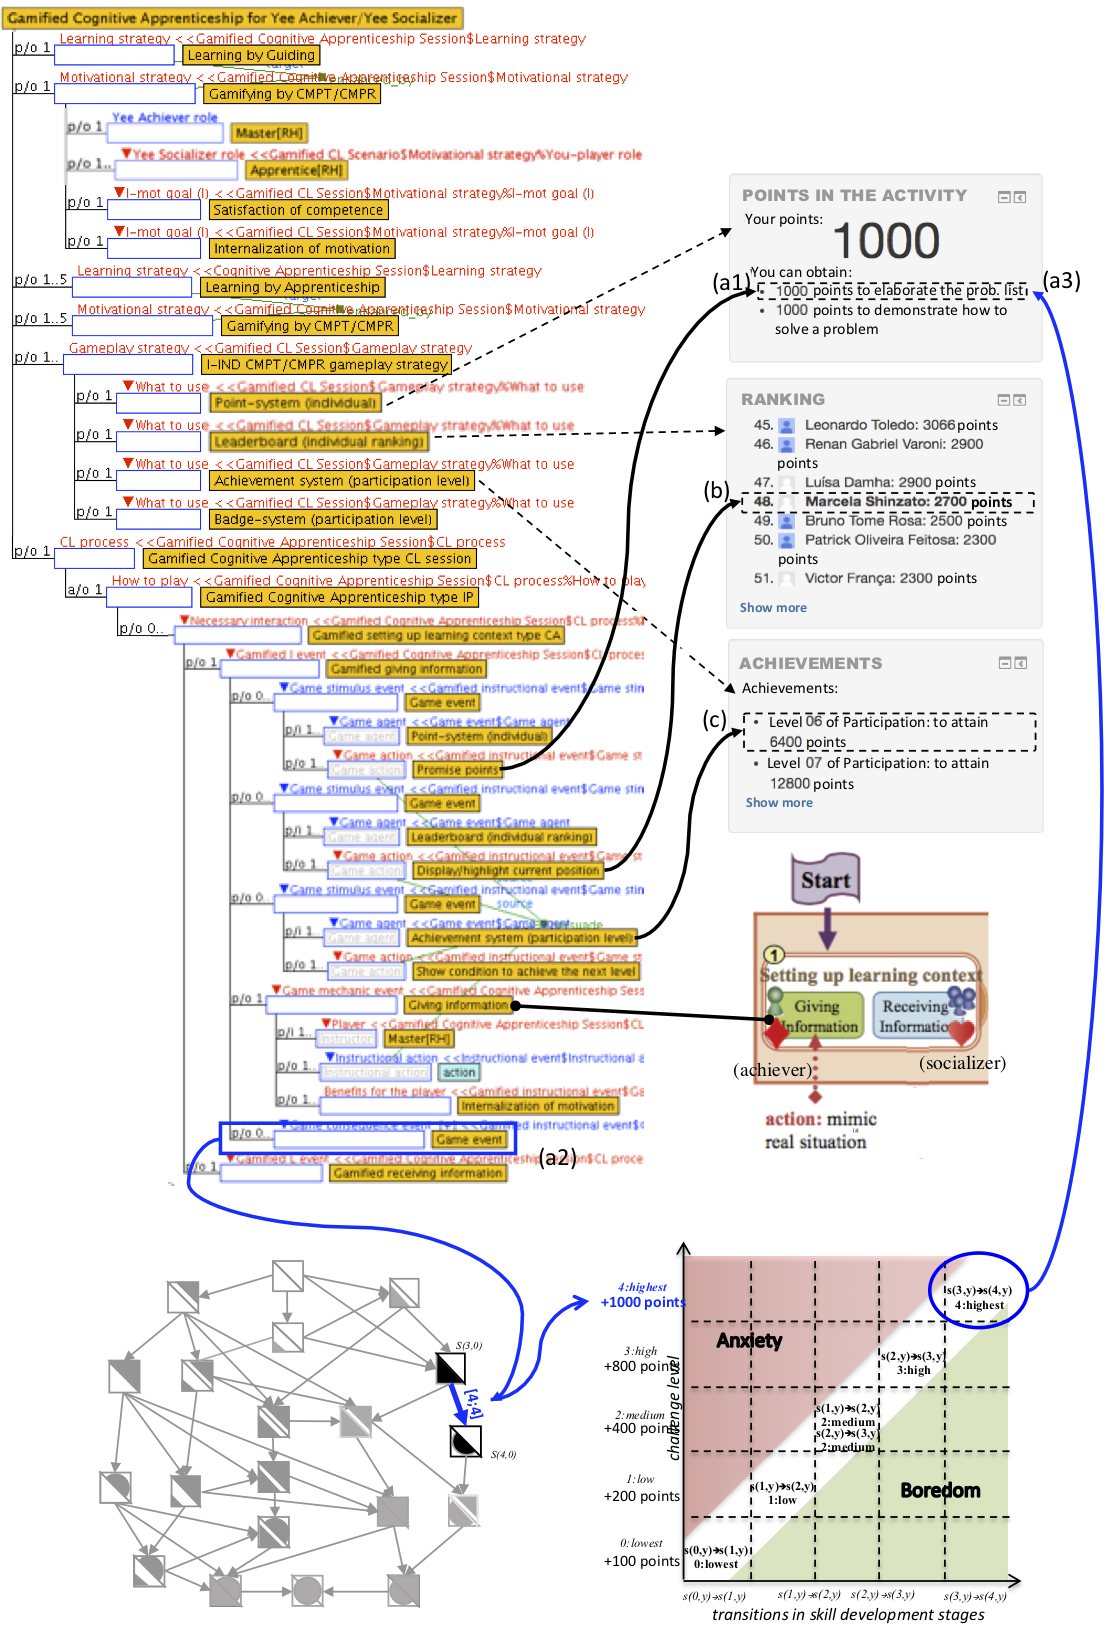
\includegraphics[width=0.8\textwidth]{images/chap-mechanisms-procedures/design-cl-gameplay.png}
 \fautor
\end{figure}

\newpage
%As we mentioned in the previous section, persuasive game design models [24, 30] are the information source to define the Gamified influential I_L events in gamified CL scenarios. Currently, in the ontology OntoGaCLes, the Persuasive Game Design Strategies (PGDSs) proposed by Orji et al. [24] have been applied in the CL process of CL scenarios based on the Cognitive Apprentice theory, and these PGDSs have been personalized for achievers using the Yee’s model. Fig 5(d) shows part of the ontological structure formalized using the PGDSs to represent the event “Gamified setting up learning context” in which the instructional event “Gamified Giving information” has as stimulus three game events defined for game actions: promise points, display/highlight current position, and show condition to achieve the next level. These game actions are defined to persuade the master student to perform the instructional action “mimic real situation” defined in the instructional event “Giving information.” Furthermore, the gamified I_L event “Gamified setting up learning context” defines that the game actions will be respectively done by the game agents: a point system with individual points, a leaderboard with an individual ranking, and the achievement system for participation level. Finally, the expected benefit for the master student is the internalization of motivation (benefits for the player) as shown in Fig 5(d).

\subsection*{Step (3): Interaction Analysis}

Although the game elements are introduced and set-up in a CL session to to change peoples’ attitudes, intentions, motivations and/or behaviors through the whole CL process, there is no guarantee that these change occurred during the execution of gamifed CL sessions. Therefore, after the execution of a gamified CL session obtained by intelligent theory-aware systems that uses the ontology OntoGaCLeS, it is necessary to understand what changes occurred while the gamified CL scenario was executed in the learning environment. In this sense, an \emph{interaction analysis} should be carried out with the data gathered from the virtual learning environment in which the gamified CL sessions was executed to identify whether the designed changes occurred satisfactorily. To enable computers to support such a task, it is necessary to use the ontological structures that represent the desired changes in the gamified I\_L events, and the changes in real interactions. By doing so, computers can compare the difference between the changes indicated by the ontological structures and the real interactions which helps to create a metric to measure the benefits of gamification and to improve the modeling of gamified I\_L events.

%(2) Design the CL Gameplay

%In the step (1), the designer sets the proper player roles and game elements for each student. In the step (2), he/she designs the CL gameplay as a set of CL game dynamics employing the player roles and game elements that were setting in the first phase. Final-ly, in the step (3), the designer makes an interaction analysis over the obtained gamified CL scenarios to propose better solutions by the meaningful result obtained during the run-time of CSCL scripts.
 
%Fig.1. Flow to gamify a CL scenario in an intelligent theory-aware system. In previous works [2, 4, 5], we define ontological structures that allow us to accomplish the step (1) by the building of models that personalize gamification based on the individual differences of students, such as cur-rent motivation stages, psychological needs and individual personality preferences. To accomplish the step (2), the work [3] propose a set of ontological structures to represent the application of PSs in CL scenarios. To establish these structures employing concepts and semantic relations in our ontology, we use the ontology engineering techniques [24], the Hozo Ontology editor [21], and the model of roles proposed by Mizogu-chi, R. et al. [26].


% The ont-gamified CL sessions have been gamified according to the suggestions given by intelligent-theory aware systems, which in turn used the ontology OntoGaCLeS as information source to give these suggestions. 

%\newpage
%%%%%%%%%%%%%%%%%%%%%%%%%%%%%%%%%%
\section[Reference Architecture of Intelligent-theory Aware Systems]{Reference Architecture of Intelligent-theory Aware Systems that Use the Ontology OntoGaCLeS}
\label{sec:reference-architecture}

\autoref{fig:reference-architecture} shows the proposed reference architecture for building the next generation of intelligent systems, referred to as intelligent theory-aware systems, that can be created and used to deal with the motivation problem by the gamification of CL sessions. This reference architecture aims to help two stakeholders, \emph{instructional designer} and \emph{gamify expert}, to accomplish their activities in two different environments denominated \aspas{\emph{Intelligent theory-aware authoring environment}} and \aspas{\emph{Gamification-framework editing environment}.}

\begin{figure}[htb]
 \caption{A reference architecture of intelligent theory-aware systems to gamify CL sessions}
 \label{fig:reference-architecture}
 \centering
 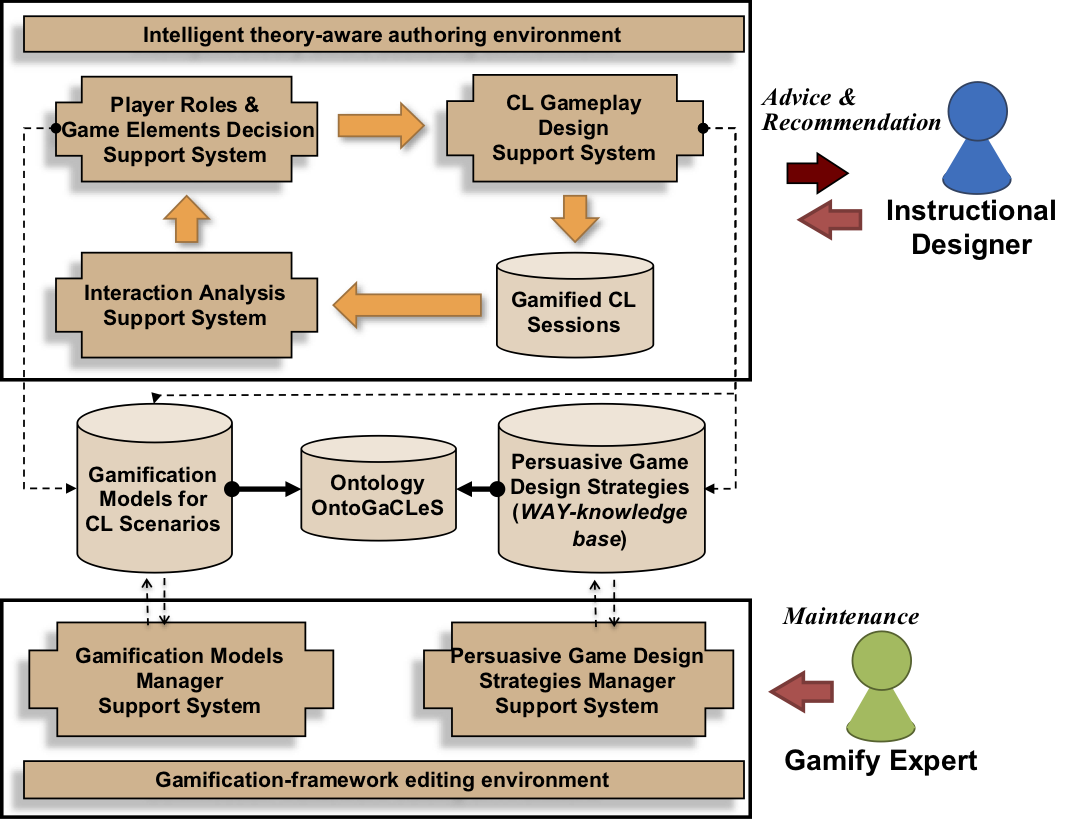
\includegraphics[width=1\textwidth]{images/chap-mechanisms-procedures/reference-architecture.png}
 \fautor
\end{figure}

\noindent
\textbf{Intelligent Theory-aware Authoring Environment}: An environment developed to provide advices and recommendations to help the instructional designer to gamify CL sessions, so that it is composed by three intelligent theory-aware systems, each one of them developed to support one of these step defined in the proposed conceptual flow to gamify CL sessions (\autoref{sec:conceptual-flow-gamify-cl-sessions}). In this sense, this environment is composed by the following support-systems:
\begin{itemize}
\item A \emph{Player Roles \& Game Elements Decision Support System} - as a system that analyzes the profile data of participants in the CL session, and based on this data, helps the instructional designer can make decisions about the player roles that will be assigned for those participants, and which game elements should be introduced in the learning environment to deal with the motivation problem;

\item A \emph{CL Gameplay Design Support System} - as a system that, based on the player roles and game elements assigned for the participants of a CL session, provides suggestions to define the interactions between the game elements and participants.

\item A \emph{Interaction Analysis Support System} - as a system that, after the execution of gamified CL session, helps the instructional designer to identify whether the designed interactions between the game elements and participants satisfactorily occurred. Thereby, this system requires a Log data that contains information related to the execution of gamified CL sessions in the learning environment.
\end{itemize}

\noindent
\textbf{Intelligent Theory-aware Authoring Environment:} An environment in which the gamify expert is supported in the maintenance (creation/update) of ontology-based gamification models for CL scenarios, and the WAY-knowledge base of game design and persuasive game design strategies. Thus, this environment is composed by two support-system:
\begin{itemize}
\item A \emph{Gamification Models Manager Support System} - as a system that helps the gamify expert to create and update ontology-based gamification models for CL scenarios. 
These models are: ontological models to personalize the gamification of CL scenarios (detailed in \autoref{chapter:ontogacles-1}), and ontological models to apply gamification as persuasive technology (detailed in \autoref{chapter:ontogacles-2}).

\item A \emph{Persuasive Game Design Strategies Manager Support System} - as a system developed to support the maintenance of game design strategies, persuasive game design strategies, and gameplay scenario model.
\end{itemize}

%The next subsections present the prototypes that are being built based on the reference architecture presented above. Rather than shown the complete functionalities of these systems, the purpose is to show some of them to demonstrate the usefulness of the ontology OntoGaCLeS, the GIMF model, and the \autoref{algorithm:set-player-roles-game-elements}.

%\subsection[Intelligent Theory-aware Authoring Environment]{Intelligent Theory-aware Authoring Environment for the Moodle Platform}
%\label{subsec:autoring-moodle-platform}

%, and it is composed by one ccording to the reference architecture (\autoref{fig:reference-architecture})

%\subsubsection*{Player Role \& Game Elements Decision Support System: }

%\subsubsection*{CL Gameplay Design Support System: }

%during (a) group formation, (b) the design of CL activities, (c) the recommendation of learning materials, (d) the
%analysis of individual and group outcomes, and (e) the identification of a learner’s stage of
%development. The aim is to support the design of CL sessions based on learners’ conditions,
%desires, and requirements. All of these systems are empowered with ontologies to support their reasoning, and provide the 

%propose to set player roles and game elements for the participants of a CL session


%group formation to create computational programs that can help users design theory-based CL scenarios.  not to demonstrate  main idea behind the development of these prototypes is shown 


%T shown in \autoref{fig:reference-architecture}.  levels of guidance during (a) group
%formation, (b) the design of CL activities, (c) the recommendation of learning materials, (d) the analysis of individual and group outcomes, and (e) the identification of a learner’s stage of development.  The aim is to support the design of CL sessions based on learners’ conditions, desires, and requirements. All of the sub-systems of CHOCOLATO are empowered with ontologies to support their reasoning.



%The first prototype will concentrate only on the CL design support system through the use of GMIP. The second prototype will be more comprehensive and show a web-based tool that semi-automatically supports group formation and the designing of CL activities for specific domains.




%\subsection{Gamification-framework Editing Environment for the ALD tool}
%\label{subsec:editing-ald-tool}

%to provide support in the gamification of CL scenarios

%a reference architecture based on this flow to build computer-based mechanisms that provide support in intelligent-theory aware systems for dealing with the motivation problem caused by the scripted collaboration


%reference architecture for semantic-web intelligent theory-aware systems that will employ the ontology OntoGaCLeS


%\begin{landscape}
%\begin{figure}[htb]
% \caption{Gamification framework editing environment}
% \label{fig:gamification-framework-editing-environment}
% \centering
% 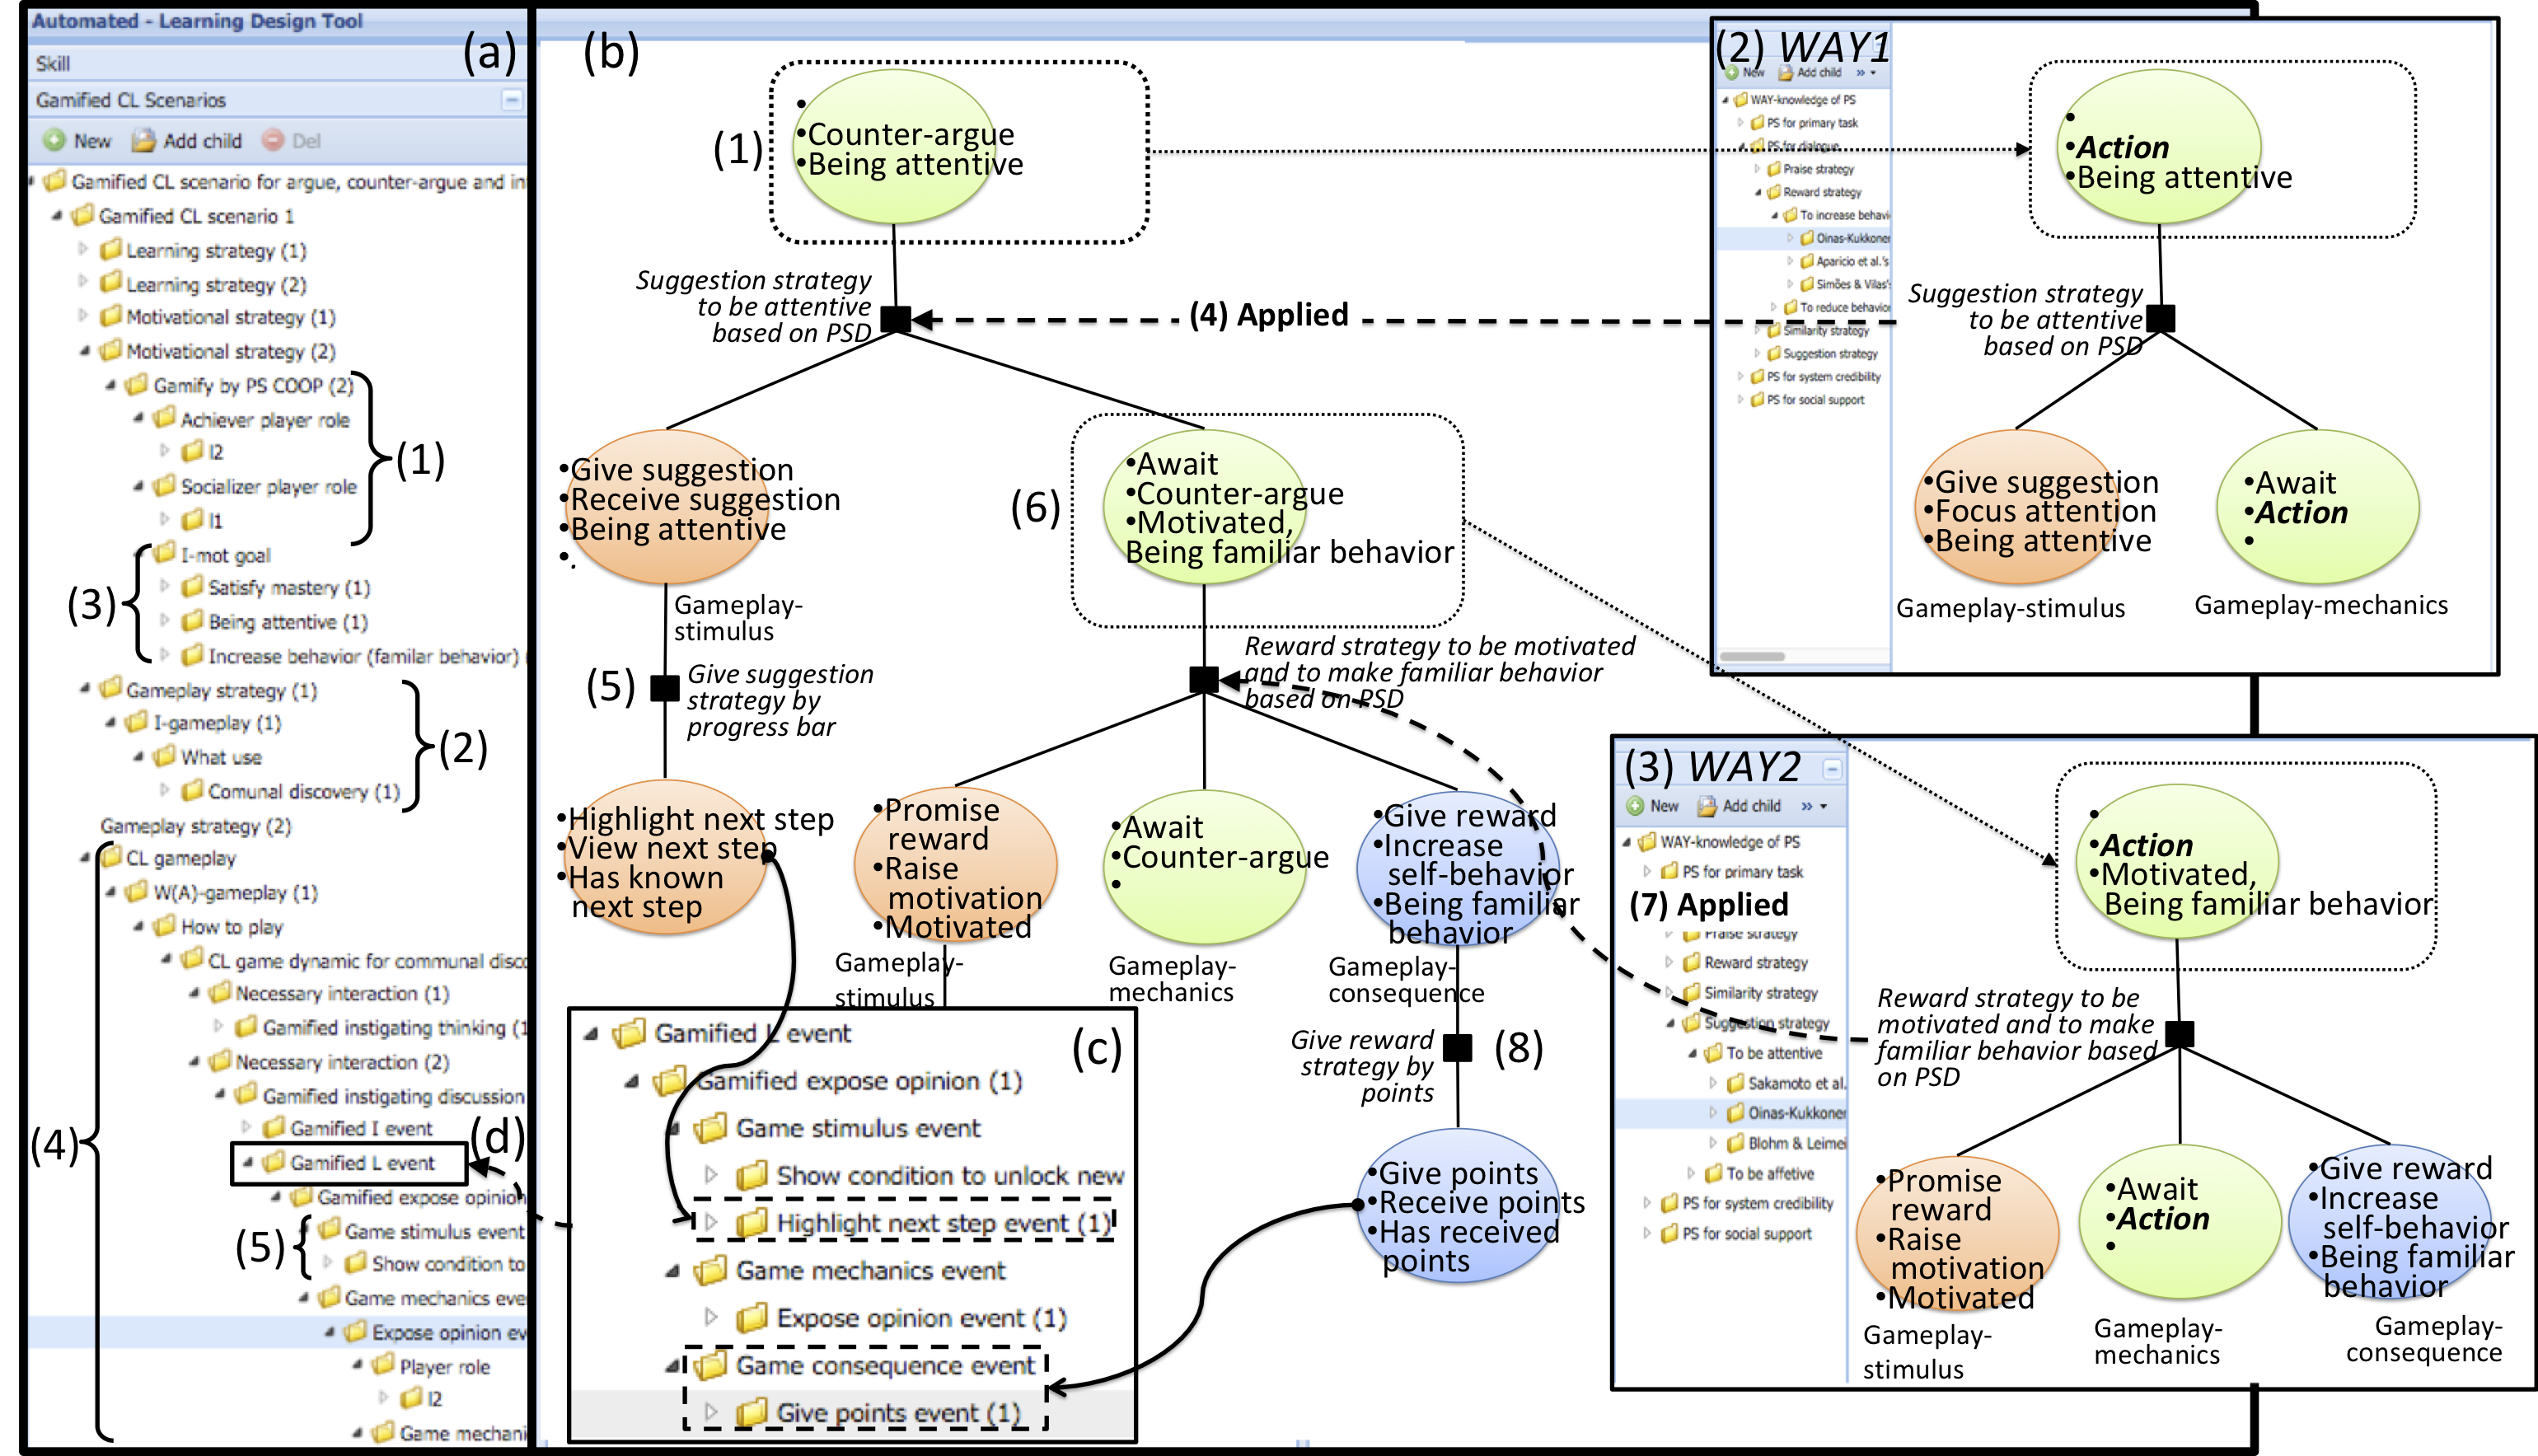
\includegraphics[width=1.5\textwidth]{images/chap-mechanisms-procedures/gamification-framework-editing-environment.png}
% \fautor
%\end{figure}
%\end{landscape}


%To demonstrate the utility of our approach that consists of the concep-tualization of PSs presented in the previous section, we are developing an advanced authoring intelligent theory-aware system based on the refer-ence architecture shown in Fig. 4. Fig. 9 illustrates the manner in which this theory-aware system uses the WAY-knowledge base of PSs to gam-ify a CL scenario during the CL gameplay design. In this example, as we show in Fig. 9 (a), the CL scenario being gamified is a scenario based on the CSCL script for “argumentation, counter-argumentation and inte-gration” proposed by Stegmann et al. in [33]. After the selection of player roles and games elements for each student of CL scenario, as shown in Fig. 9 (a-1), the socializer role is assigned for the student l1 who has the role of arguer, while the achiever role is assigned for the student l2 who has the role of co-arguer. Fig. 9 (a-1) also shows that the motivational strategies for socializers and achievers are the “Gamifying by persuasive strategy COOP,” in both cases. Fig. 9 (a-2) shows that the selected game elements in gameplay strategy (I-gameplay strategy) for socializer and achiever are the communal discovery. Finally, the individual motivation goals (I-mot goal) for students l2 are “satisfy mastery,” “be attentive” and “increase behavior (familiar behavior)” as shown in Fig 9 (a-3).
  
%Fig. 9. Illustration of how to employ the WAY-knowledge base of Persuasive Strategies.
%The default “CL gameplay” for the scenario shown in Fig. 9 (a-4) is obtained by employing an ontological model that extends the ontological structures shown in Fig. 3. This model employs the information defined by Orji et al. in [29], and its detail of construction can be found in [3]. As result of the application of this model, each gamified instructional and learning event defines the game action “show condition to unlock new content” as game stimulus event that persuades the student l2 to do the actions of learning event as shown in Fig. 9 (a-5).
%Employing the WAY-knowledge base of PSs, we can personalize the gamified instructional and learning event for each student of a gamified CL scenario by adding new game stimulus and game consequences events, so that the Fig. 9 (b) shows how this personalization is done for the student l2 over the learning event “expose opinion.” First, after the selection of the event that will be personalized, the macro-gameplay event is automatically filled by the information of selected event as shown in Fig. 9 (b-1). Based in the individual motivational goals “be attentive” and “increase behavior (familiar behavior)” of student l2, the system pro-poses the ways of decomposition WAY1 and WAY2, respectively shown in Fig. 9 (b-2) and Fig. 9 (b-3). The first way (WAY1) emerges from the PS “Oinas-Kukkonen & Harjumaa’s suggestion strategy to be attentive” because it allows to “be attentive” (I-mot goal). The second way (WAY2) emerges from the PS “Oinas-Kukkonen & Harjumaa’s reward strategy to increase behavior” because it allows to “increase behavior (familiar behavior).” In this example, the designer selects the first way (WAY1) decomposing the macro-gameplay (Fig. 9 (b-1)) into two micro-gameplay events with the game actions “give suggestion” and “awaiting action” as shown in Fig. 9 (b-4). The designer can decompose the game action “give suggestion” by employing different PSs. For this example, the designer selects the PS “Orji et al.’s suggest by progress bar” as shown in Fig. 9 (b-5). Next, the designer decomposes the gameplay me-chanics event shown in Fig. 9 (b-6) into two micro-gameplay events with the game actions “awaiting action” and “give reward” as shown in Fig. 9 (b-7). This decomposition emerges from the PS “Oinas-Kukkonen & Harjumaa’s reward strategy to increase behavior” (WAY2) shown in Fig. 9 (b-3). Finally, the game action “give reward” is decomposed into the game action “give points” by the application of PS “Orji et al.’s re-ward by points” shown in Fig. 9 (b-8).
%The process to personalize the gamified instructional and learning event shown in Fig. 9 (b) can be repeated for each student and over each instructional and learning event to define a better gamified CL scenario. At the end of this process, as shown in Fig. 9 (c), the system integrates the game events in a set of game stimulus and game consequence events. For this example, the game action “highlight next step” done by the “progress bar system” is integrated into a game stimulus event, and the game action “give points” done by the “point system” is integrated in a game consequence event. Finally, the last step is the addition of game stimulus and game consequence events into its respective gamified event as shown in Fig. 9 (d).




